\chapter{速度运动学与静力学 (Velocity Kinematics and Statics)}

在前向运动学（位置映射）的基础上，第五章研究关节速度 $\dot{\theta}$ 与末端执行器运动旋量 $\mathcal{V}$ 之间的线性映射关系。

\section{雅可比矩阵 (The Manipulator Jacobian)}

雅可比矩阵 $J(\theta) \in \mathbb{R}^{6 \times n}$ 描述了末端速度对关节速度的线性敏感度。根据参考系的选择，分为空间雅可比和物体雅可比。

\subsection{空间雅可比矩阵 $J_s(\theta)$}

\begin{formulabox}{空间雅可比定义}
\begin{equation}
    \mathcal{V}_s = J_s(\theta)\dot{\theta}
\end{equation}
其中第 $i$ 列 $J_{si}$ 是当只有关节 $i$ 运动时，在固定系 $\{s\}$ 下观察到的瞬时螺旋轴：
\begin{equation}
    J_{si}(\theta) = [Ad_{e^{[\mathcal{S}_1]\theta_1} \dots e^{[\mathcal{S}_{i-1}]\theta_{i-1}}}] \mathcal{S}_i
\end{equation}
\end{formulabox}

\begin{center}
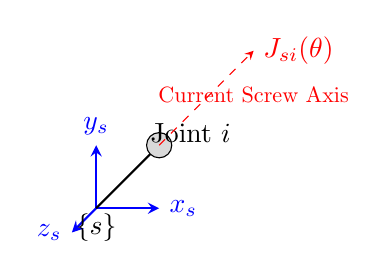
\begin{tikzpicture}[scale=0.8, >=stealth]
    % Draw Space Frame
    \draw[->, thick, blue] (0,0,0) -- (1,0,0) node[right]{$x_s$};
    \draw[->, thick, blue] (0,0,0) -- (0,1,0) node[above]{$y_s$};
    \draw[->, thick, blue] (0,0,0) -- (0,0,1) node[left]{$z_s$};
    \node at (0,-0.3) {$\{s\}$};
    
    % Draw Robot Link 1
    \draw[thick] (0,0) -- (1,1);
    \draw[fill=gray!30] (1,1) circle (0.2);
    \node at (1.5,1.2) {Joint $i$};
    
    % Draw Current Screw Axis
    \draw[dashed, red, ->] (1,1) -- (2.5,2.5) node[right]{$J_{si}(\theta)$};
    \node[text=red, scale=0.8] at (2.5,1.8) {Current Screw Axis};
\end{tikzpicture}
\end{center}

\subsection{物体雅可比矩阵 $J_b(\theta)$}

\begin{formulabox}{物体雅可比定义}
\begin{equation}
    \mathcal{V}_b = J_b(\theta)\dot{\theta}
\end{equation}
其第 $i$ 列 $J_{bi}$ 是在物体坐标系 $\{b\}$ 下观察到的瞬时螺旋轴。
\end{formulabox}

\begin{mybox}{两者转换关系}
空间雅可比与物体雅可比通过伴随矩阵转换：
\begin{equation}
    J_s(\theta) = [Ad_{T_{sb}}] J_b(\theta), \quad J_b(\theta) = [Ad_{T_{bs}}] J_s(\theta)
\end{equation}
\end{mybox}

\section{开链静力学 (Statics of Open Chains)}

雅可比矩阵不仅描述速度映射，也描述了末端力旋量 $\mathcal{F}$ 与关节力矩 $\tau$ 之间的平衡关系。

\begin{mybox}{虚功原理推导 (Principle of Virtual Work)}
考虑功的标量特性，关节空间功率应等于末端空间功率：
\begin{equation}
    \tau^T \dot{\theta} = \mathcal{V}^T \mathcal{F} = (J\dot{\theta})^T \mathcal{F} = \dot{\theta}^T J^T \mathcal{F}
\end{equation}
由于该式对任意 $\dot{\theta}$ 均成立，得：
\begin{equation}
    \tau = J^T(\theta) \mathcal{F}
\end{equation}
\end{mybox}

\section{奇异性分析 (Singularity Analysis)}

当 $J(\theta)$ 的秩（Rank）小于其最大可能秩时，称机械臂处于**奇异位形**。

\begin{itemize}
    \item \textbf{丢失自由度}：在某些方向上无法产生线速度或角速度。
    \item \textbf{无限大力矩}：在奇异方向施加力时，可能需要无限大的关节力矩。
\end{itemize}

\section{可操作性 (Manipulability)}

可操作性椭球用于量化机器人在当前位形下的运动能力。

\begin{formulabox}{可操作性指标}
定义单位关节速度集合 $\|\dot{\theta}\| \le 1$，映射到末端空间得到：
\begin{equation}
    \mathcal{V}^T (J J^T)^{-1} \mathcal{V} \le 1 \quad \text{(速度椭球)}
\end{equation}
\textbf{吉川指标 (Yoshikawa's Measure)}：$\mu = \sqrt{\det(J J^T)} = \sigma_1 \sigma_2 \dots \sigma_m$。
\end{formulabox}

\begin{center}
\begin{tikzpicture}[scale=1.2]
    % Draw Ellipse
    \draw[thick, blue, rotate=30] (0,0) ellipse (1.5cm and 0.6cm);
    \draw[->, thick] (0,0) -- (1.3,0.75) node[above right]{$\sigma_1$};
    \draw[->, thick] (0,0) -- (-0.3,0.5) node[left]{$\sigma_2$};
    \node at (0,-1) {速度可操作性椭球 (Velocity Ellipsoid)};
    
    % Draw Singularity case
    \begin{scope}[xshift=5cm]
        \draw[thick, red] (-1.5,0) -- (1.5,0);
        \draw[->, thick] (0,0) -- (1.2,0) node[below]{$\sigma_1$};
        \draw[->, thick, gray] (0,0) -- (0,0.1) node[above]{$\sigma_2 \to 0$};
        \node at (0,-1) {奇异位形下的塌缩};
    \end{scope}
\end{tikzpicture}
\end{center}

\begin{mybox}{速度与力的对偶性}
速度椭球的长轴方向是运动最灵敏的方向，同时也是力输出能力最弱的方向（力椭球的短轴）。
\end{mybox}

